\documentclass[11pt]{article}

% ----------------------------------------------------------------------------
% Urban Mobility Equity Dashboard --- MS Project Report, Full Draft (Ch. 1--5)
% Styled to match the EMGT 7945 proposal. Compile: tectonic Full_Draft_Ch1-5.tex
% ----------------------------------------------------------------------------

\usepackage[letterpaper,margin=1in]{geometry}
\usepackage[T1]{fontenc}
\usepackage[utf8]{inputenc}
\usepackage{amsmath}
\usepackage{newtxtext,newtxmath}  % Times for BOTH text and math (consistent, embedded)
\usepackage{microtype}
\usepackage{graphicx}
\usepackage{booktabs}
\usepackage{array}
\usepackage{tabularx}
\usepackage{enumitem}
\usepackage{titlesec}
\usepackage{caption}
\usepackage[hidelinks]{hyperref}
\usepackage{fancyhdr}
\usepackage{xcolor}

\graphicspath{{../data/outputs/figures/}}
\definecolor{neunavy}{RGB}{21,51,79}

\titleformat{\section}{\large\bfseries\color{neunavy}}{\thesection.}{0.5em}{\MakeUppercase}
\titleformat{\subsection}{\normalsize\bfseries}{\thesubsection}{0.5em}{}
\titlespacing*{\section}{0pt}{14pt}{6pt}
\titlespacing*{\subsection}{0pt}{8pt}{3pt}

\setlength{\parskip}{5pt}
\setlength{\parindent}{0pt}
\newcolumntype{Y}{>{\raggedright\arraybackslash}X}

\pagestyle{fancy}
\fancyhf{}
\rhead{\small Urban Mobility Equity Dashboard}
\lhead{\small EMGT 7945}
\rfoot{\small\thepage}

\captionsetup[table]{labelfont=bf,font=small,skip=4pt}
\captionsetup[figure]{labelfont=bf,font=small,skip=4pt}

\begin{document}

% ----------------------------- Title block -----------------------------
\thispagestyle{empty}
\begin{center}
{\large\bfseries MS PROJECT --- FINAL REPORT (CHAPTERS 1--5)}\\[2pt]
{\normalsize EMGT 7945 MS Project}\\[18pt]
{\LARGE\bfseries\color{neunavy} Urban Mobility Equity Dashboard:}\\[4pt]
{\Large\bfseries\color{neunavy} Mapping Who Gets Left Behind in U.S. Cities}\\[22pt]
\end{center}

\begin{center}
\renewcommand{\arraystretch}{1.3}
\begin{tabular}{r l}
\textbf{Submitted by} & Aashritha Krishna Kanagala \\
\textbf{Program} & Master of Science in Engineering Management (MSEM) \\
\textbf{Course} & EMGT 7945 MS Project \\
\textbf{University} & Northeastern University, Boston, Massachusetts \\
\textbf{Supervisor} & Professor Sivarit (Tony) Sultornsanee \\
\textbf{Date} & August 2026 \\
\end{tabular}
\end{center}

\vspace{14pt}
\textbf{\color{neunavy} Abstract.}\quad
Urban mobility infrastructure --- public transit, walkable streets, bicycle
facilities, and electric-vehicle (EV) charging --- is unevenly distributed, yet
existing measurement tools treat each dimension in isolation. This project
constructs a \emph{Mobility Equity Score} (MES): a transparent, reproducible
composite index that integrates all four dimensions at the U.S. Census-tract
level, and applies it to three structurally distinct cities (Chicago, Houston,
Seattle) using only open data. Across all three cities the MES exhibits strong,
significant spatial clustering (global Moran's $I = 0.82$--$0.92$) and is
\emph{positively} associated with the share of zero-vehicle and renter
households, reflecting that supply-side infrastructure concentrates in dense,
central tracts. The bivariate \emph{negative} association with median income is
largely accounted for by urban form: after controlling for population density
and distance to the central business district --- and after spatial-regression
correction for the strong spatial dependence --- it attenuates to
non-significance in Houston, reverses weakly in Chicago, and persists only in
Seattle. The results are therefore interpreted as \emph{associational} and
consistent with a supply--\emph{need} mismatch (need proxied by car-free and
renter households), not as evidence of a causal relationship. The methodology is
released as an open-source pipeline and an interactive dashboard so any city with
open data can reproduce the analysis.

\vspace{6pt}
{\hypersetup{linkcolor=black}
\renewcommand{\contentsname}{\normalsize\bfseries Table of Contents}
\tableofcontents}
\newpage

% ============================== CHAPTER 1 ==============================
\section{Introduction and Motivation}

\subsection{Background}
Transportation is a fundamental determinant of economic opportunity in urban
America. A person's ability to reach employment, healthcare, education, and
essential services depends on a layered ecosystem of infrastructure: transit
frequency and coverage, pedestrian networks, bicycle facilities, and access to
electric-vehicle (EV) charging. Each dimension has documented equity gaps.
Transit deserts disproportionately affect low-income and minority
communities~\cite{aman2020,maharjan2024}; walkability is highly racialized, with
communities of color inhabiting systematically less walkable
neighborhoods~\cite{urban2022}; disadvantaged communities have roughly 64\% fewer
public EV chargers per capita~\cite{lou2025}; and bicycle infrastructure remains
underfunded in lower-income areas~\cite{ahmed2024}. Despite this evidence, the
available measurement tools remain siloed --- the EPA National Walkability Index,
the DOE Alternative Fuels Station Locator, the FTA National Transit Database, and
OpenStreetMap bicycle data each capture one dimension in isolation.

\subsection{Problem Statement}
\begin{sloppypar}
Low-income and minority neighborhoods may experience \emph{compounded},
multi-dimensional mobility disadvantage --- scoring poorly across several
dimensions at once rather than in a single dimension. The magnitude of this
compounding, and where it is most severe, have not been quantified in an
integrated, reproducible framework. Equally unexamined is the \emph{direction} of
the supply-side relationship: whether infrastructure is scarcest where
demand-side need (car-free, low-income households) is greatest, or whether it
instead concentrates in dense cores for reasons of land use and density. Both
questions impede evidence-based infrastructure-investment decisions.
\end{sloppypar}

\subsection{Research Questions}
The project is framed around one central question and four measurable
sub-questions. Each sub-question names the specific quantity, statistical test,
and decision criterion used to answer it (developed in Chapter~3).

\begin{enumerate}[leftmargin=1.5em,itemsep=2pt,label=\textbf{RQ\arabic*.}]
\item \textbf{(Measurement.)} Can four heterogeneous open datasets be integrated
into a single tract-level composite (MES) whose components are related but
non-redundant (inter-sub-index correlations reported) and whose downstream
findings are stable under alternative weighting schemes (sign and significance
unchanged across equal, entropy, PCA, and policy-priority weights)?
\item \textbf{(Distribution.)} What share of tracts in each city are mobility
deserts (MES below the 25th percentile) and compounded deserts (bottom quartile
in $\geq 2$ sub-indices), and is that classification robust to the threshold
(Jaccard overlap $\geq 0.75$ across the 20th/25th/30th percentiles)?
\item \textbf{(Equity.)} What is the sign, magnitude ($|r|$), and significance
($p < 0.05$, 95\% CI excluding zero) of the association between the MES and each
of median income, percent non-white, percent zero-vehicle, and percent renter?
\item \textbf{(Spatial structure and typology.)} Do MES values cluster spatially
(global Moran's $I$, $p < 0.05$), where are the statistically significant
low-low cold spots (local Moran's $I$), and how many distinct mobility
``profiles'' (K-means, silhouette-selected $k$) recur across neighborhoods?
\end{enumerate}

\subsection{Objectives}
\begin{enumerate}[leftmargin=1.5em,itemsep=2pt,label=\textbf{O\arabic*.}]
\item Construct the MES from four equally-weighted, 0--100-normalized
sub-indices at the census-tract level for three Phase-1 cities, with documented
indicator selection and normalization.
\item Quantify the association between the MES and four socioeconomic indicators
with effect sizes, $p$-values, and confidence intervals.
\item Classify and rank mobility deserts and compounded deserts, and validate the
classification against threshold and weighting sensitivity.
\item Characterize the spatial structure (Moran's $I$/LISA) and the recurring
neighborhood mobility typologies (K-means).
\item Release a reproducible open-source pipeline and an interactive dashboard
for dissemination and replication.
\end{enumerate}

\subsection{Research Contributions}
The contribution of this work is \emph{methodological and empirical}, not the
visualization system (the dashboard is a dissemination layer over the analysis,
not the result). Specifically:
\begin{enumerate}[leftmargin=1.5em,itemsep=1pt]
\item \textbf{An integrated composite.} The first open, reproducible integration
of transit, walkability, bicycle, and EV-charging supply into a single
tract-level index, where prior tools measure one dimension or one scale (Sec.~2.7).
\item \textbf{A transparent, tested methodology.} Every modeling choice ---
indicator selection, within-city min--max normalization, equal-weight baseline,
and desert thresholds --- is stated and stress-tested through weighting
(equal/entropy/PCA/AHP) and threshold (20/25/30th percentile) sensitivity
analyses, addressing the reproducibility and value-ladenness concerns raised for
composite indicators~\cite{nardo2008}.
\item \textbf{An empirical finding.} Across three structurally different cities,
supply-side mobility infrastructure concentrates in dense, central tracts that
tend to be higher-renter and car-free. The bivariate negative association with
income is shown to be largely an \emph{urban-form artifact} (it does not survive
density/centrality controls or spatial regression, except in Seattle) ---
reframing the equity question, associationally, as a supply--\emph{need}
mismatch rather than a simple ``poor areas are under-served'' narrative (Sec.~5).
\item \textbf{A replication artifact.} A documented Python pipeline (MIT-licensed)
that reproduces the entire analysis for any U.S. city with open data.
\end{enumerate}

\subsection{Organization}
Chapter~2 critically reviews prior work and isolates the gap. Chapter~3 specifies
the methodology. Chapter~4 presents results. Chapter~5 discusses findings,
implications, limitations, and future work.

% ============================== CHAPTER 2 ==============================
\section{Literature Review}

Rather than summarizing studies individually, this chapter organizes prior work
by what it measures and how, then isolates the specific gap the MES fills
(Table~\ref{tab:gap}).

\subsection{Single-Dimension Equity Measurement}
The strongest body of evidence is \emph{single-dimension}. In transit, Aman and
Smith-Colin~\cite{aman2020} operationalize ``transit deserts'' as a
tract-level supply--demand gap from GTFS, and Maharjan et al.~\cite{maharjan2024}
confirm the pattern nationally; both establish that low-income and minority
tracts are under-served --- consistent with evidence that transit access
directly shapes job accessibility~\cite{ermagun2020} --- but neither places
transit alongside other modes.
Walkability research standardizes on the EPA National Walkability
Index~\cite{epa2024} and documents racialized disparities~\cite{urban2022}, while
active-travel toolkits~\cite{albashir2024,sustrans2023} refine walk/bike access
but again in isolation. EV-charging equity is the newest strand: Lou et
al.~\cite{lou2025} and Chen and Li~\cite{chenli2024} demonstrate severe
under-provision for disadvantaged and renter households. The common limitation is
\emph{dimensional siloing}: each literature answers ``is mode $X$ inequitable?''
but none answers ``which neighborhoods are disadvantaged across modes at once?''

\subsection{Composite Indicators and Their Critique}
Composite indicators are attractive for communication but contested on
methodology. The OECD/JRC handbook~\cite{nardo2008} warns that normalization and
weighting are value judgments that must be paired with sensitivity analysis ---
a discipline frequently omitted in applied indices. This project treats that
critique as a design requirement (Secs.~3.6--3.7) rather than an afterthought,
distinguishing it from single-shot composites.

\subsection{Existing Integrated Tools --- and Why They Fall Short}
The closest comparators are multi-dimensional tools, but each trades away
tract-level, multi-modal, or open-data properties. The EPA Smart Location
Database is multi-variable but built for walkability/location efficiency, not
transit/bike/EV equity. The Urban Institute SITE tool~\cite{urbanSITE2025}
measures infrastructure \emph{spending} equity, not physical supply. The Oliver
Wyman Urban Mobility Readiness Index~\cite{oliverwyman2024} ranks whole cities,
not neighborhoods. Pandey et al.~\cite{pandey2025} link urbanization to widening
infrastructure inequality but at national/global scale. Table~\ref{tab:gap}
summarizes the comparison.

\begin{table}[htbp]
\centering
\caption{Critical comparison of representative prior work. The MES is the only
approach that is simultaneously multi-modal (all four dimensions), tract-level,
open-data, and demographically cross-referenced.}
\label{tab:gap}
\small
\begin{tabularx}{\textwidth}{l c c c c}
\toprule
\textbf{Prior work} & \textbf{Dimensions} & \textbf{Spatial unit} & \textbf{Open data} & \textbf{Demographic cross-ref} \\
\midrule
Transit-desert models \cite{aman2020,maharjan2024} & Transit only & Tract & Yes & Yes \\
EPA walkability \cite{epa2024,urban2022} & Walk only & Block group & Yes & Partial \\
EV-charging equity \cite{lou2025,chenli2024} & EV only & Tract/ZIP & Yes & Yes \\
Bikeability indices \cite{ahmed2024,albashir2024} & Bike only & Varies & Yes & Partial \\
Urban Institute SITE \cite{urbanSITE2025} & Spending (multi) & City/region & Partial & Yes \\
Oliver Wyman UMRI \cite{oliverwyman2024} & Multi (readiness) & City & No & No \\
\textbf{This work (MES)} & \textbf{All four} & \textbf{Tract} & \textbf{Yes} & \textbf{Yes} \\
\bottomrule
\end{tabularx}
\end{table}

\subsection{Spatial and Multivariate Methods}
Because infrastructure is spatially structured, the analysis draws on established
methods: global and local Moran's $I$~\cite{anselin1995} for spatial clustering
and cold-spot detection, and K-means with silhouette
validation~\cite{rousseeuw1987} for typology discovery. These are chosen (Sec.~3.9--
Sec.~3.11) because they directly answer the distributional and structural research
questions, not merely because they are conventional.

\subsection{Synthesis of the Gap}
Three gaps motivate the MES: (i) \emph{no integrated, multi-modal, tract-level}
supply measure exists; (ii) integrated tools that do exist are either
city-scale, spending-based, or closed; and (iii) the \emph{direction} of the
supply--demographic relationship is assumed rather than measured. The MES closes
(i) and (ii) by construction and tests (iii) empirically.

% ============================== CHAPTER 3 ==============================
\section{Methodology}

\subsection{Study Area}
The unit of analysis is the 2023 U.S. Census tract. Three cities were selected
for Phase~1 to span mobility regimes (Table~\ref{tab:cities}); Phase~2 will add
Phoenix, Atlanta, and Detroit. Selection criteria: population $>300{,}000$,
complete GTFS feeds, demographic diversity, and contrasting transit-investment
histories.

\begin{table}[htbp]
\centering
\caption{Phase-1 study cities and Census FIPS codes.}
\label{tab:cities}
\small
\begin{tabularx}{\textwidth}{l l l r Y}
\toprule
\textbf{City} & \textbf{State (FIPS)} & \textbf{County (FIPS)} & \textbf{Tracts} & \textbf{Rationale} \\
\midrule
Chicago & Illinois (17) & Cook (031) & 1{,}332 & Mature high-frequency transit; diverse \\
Houston & Texas (48) & Harris (201) & 1{,}115 & Auto-oriented, sprawling; large low-income pop. \\
Seattle & Washington (53) & King (033) & 495 & Progressive transit and EV investment \\
\bottomrule
\end{tabularx}
\end{table}

\subsection{Indicator Selection and Sub-Index Definition}
Indicators were selected against three criteria: (a) \emph{construct validity}
--- each must be an accepted proxy for its dimension in the literature (Sec.~2);
(b) \emph{national open availability} at $\leq$ tract resolution for
reproducibility; and (c) \emph{supply orientation} --- each measures
infrastructure present near residents, keeping the composite conceptually
coherent. Table~\ref{tab:subindex} lists the resulting metrics.

\begin{table}[htbp]
\centering
\caption{The four MES sub-indices, their metrics, and data sources.}
\label{tab:subindex}
\small
\begin{tabularx}{\textwidth}{l c Y l}
\toprule
\textbf{Sub-index} & \textbf{Weight} & \textbf{Metric(s)} & \textbf{Source} \\
\midrule
Transit & 25\% & Stop density; AM-peak (07--09h) trips/hr; service span within 0.5 mi of centroid & GTFS \\
Walkability & 25\% & EPA National Walkability Index (areal-interpolated to tract) & EPA SLD v3 \\
Bicycle & 25\% & Dedicated bike-lane km per km$^2$ of tract land area & OpenStreetMap \\
EV charging & 25\% & Public-charger count and proximity to nearest DC-fast station & OSM (AFDC fallback) \\
\bottomrule
\end{tabularx}
\end{table}

\subsection{Data Preprocessing, Missing Values, and Assumptions}
All layers are reprojected to EPSG:4326 for storage and to EPSG:5070 (equal-area,
metres) for all distance/area computation. GEOIDs are zero-padded strings to
guarantee exact joins. The principal preprocessing challenge is
\emph{geographic-vintage mismatch}: the EPA walkability data is published on
2019-vintage block groups while the study uses 2023 tracts; a naive GEOID join
loses $\approx57\%$ of Houston's tracts. We therefore \emph{areally interpolate}
--- joining the index to 2019 block-group polygons (100\% GEOID match) and
area-weighting onto 2023 tracts, valid because the walkability index is an
intensive quantity. \textbf{Missing values} are preserved, not imputed, so gaps
remain visible; a tract missing any sub-index is excluded pairwise from that
statistic rather than zero-filled, and normalization propagates \texttt{NaN}. Key
\textbf{assumptions}: (i) supply near the tract centroid proxies residents'
access; (ii) the 0.5-mile transit buffer approximates walk-access to stops;
(iii) OSM bike/EV coverage, though community-maintained, is spatially unbiased
enough for within-city comparison (revisited as a limitation in Sec.~5.4).

\subsection{Sub-Index Computation}
Each raw metric is computed at the tract level before normalization.
\textbf{Transit.} From GTFS \texttt{stops} and \texttt{stop\_times}, AM-peak
(07:00--09:00) departures per stop are converted to trips/hour and the daily
service span (distinct hours with $\geq 1$ departure) is computed; stops are
spatially joined to a 0.5-mile (804.7\,m) buffer of each tract centroid, and the
tract's stop density (stops/km$^2$), mean AM-peak frequency, and span are each
normalized and averaged. \textbf{Walkability.} The area-weighted National
Walkability Index per tract (Sec.~3.4). \textbf{Bicycle.} From the OpenStreetMap
cyclable network extracted with OSMnx~\cite{boeing2017}, edges are retained as
dedicated infrastructure when the \texttt{highway} tag is cycleway/path/track or a
positive \texttt{cycleway} tag is present; edges are clipped to tracts by
geometric overlay and summed to bike-lane km per km$^2$ of tract land area.
\textbf{EV charging.} Public stations are spatially joined to tracts; chargers per
1{,}000 residents and the (inverted) distance from the tract centroid to the
nearest DC-fast station are each normalized and averaged. The authoritative
source is the DOE/NREL AFDC; where that API is unreachable the pipeline falls back
to OSM \texttt{amenity=charging\_station} points, a key-free lower-bound proxy
(Sec.~5.4).

\subsection{Normalization and MES Construction}
Each raw metric is placed on a common 0--100 scale by \emph{within-city}
min--max normalization,
\[
s^{\text{norm}} = \frac{x - x_{\min}}{x_{\max}-x_{\min}}\times 100,
\]
chosen over $z$-scores so scores are bounded, interpretable as ``percent of the
best-served tract in this city,'' and comparable across sub-indices. Because
normalization is within-city, the MES is a \emph{relative} measure; cross-city
\emph{levels} are therefore interpreted with caution (Sec.~5.4), while within-city
patterns and correlations are directly valid. The composite is the weighted sum
\[
\mathrm{MES} = \sum_{k} w_k\, s_k^{\text{norm}}, \qquad \sum_k w_k = 1,
\]
with an equal-weight baseline ($w_k = 0.25$), the neutral default recommended
absent strong prior information~\cite{nardo2008}.

\subsection{Weighting: Determination and Sensitivity}
The equal-weight baseline is a deliberate, stated choice, but its influence is
tested against three alternatives (Sec.~4.6): \emph{entropy} weights (from each
sub-index's dispersion), \emph{PCA} weights (first-component loadings), and
\emph{AHP-style} weights (illustrative expert priorities pending a formal Analytic
Hierarchy Process elicitation: transit 0.40, walk 0.30, bike 0.15, EV 0.15). If the sign, magnitude, and significance of the equity correlations are
stable across all four schemes, the substantive conclusions do not depend on the
weighting choice --- the criterion for RQ1.

\subsection{Mobility-Desert Classification and Threshold Validation}
A \emph{mobility desert} is a tract below its city's 25th MES percentile; a
\emph{compounded desert} is below the 25th percentile in $\geq 2$ sub-indices.
Because the 25th-percentile cut is arbitrary, it is validated by recomputing the
desert set at the 20th and 30th percentiles and reporting the Jaccard overlap
with the baseline and the demographic profile at each threshold (RQ2).

\subsection{Equity Correlation Analysis --- Justification}
Pearson correlation is used because the research question (RQ3) concerns the
\emph{linear direction and strength} of association between the continuous MES and
continuous demographic variables; it yields an interpretable effect size ($r$),
a significance test, and (via the Fisher $z$-transform) a confidence interval,
\[
z=\operatorname{arctanh}(r),\quad \mathrm{SE}=\tfrac{1}{\sqrt{n-3}},\quad
\mathrm{CI}_{95\%}=\tanh\!\big(z\pm1.96\,\mathrm{SE}\big).
\]
Spearman rank correlation is computed as a monotonic robustness variant
(reported in Sec.~4.2); it agrees in sign with Pearson across all cities.

\subsection{Spatial Autocorrelation --- Justification}
Ordinary correlation ignores that tracts are spatially embedded. Global Moran's
$I$ (queen contiguity, row-standardized, 999 permutations) tests whether the MES
is spatially clustered rather than random --- necessary because a clustered
pattern implies systematic, place-based (not idiosyncratic) inequity. Local
Moran's $I$ (LISA) then locates statistically significant low-low ``cold spots''
for targeting (RQ4).

\subsection{Cluster Analysis --- Justification}
To move beyond a single score to actionable \emph{profiles}, K-means clusters
tracts on the four standardized sub-indices; $k$ is selected by maximizing the
mean silhouette over $k\in\{2,\dots,7\}$ (with the inertia elbow reported), which
serves as internal validation of cluster quality. The resulting typology answers
``what \emph{kinds} of mobility disadvantage exist?'' --- directly supporting
differentiated policy (RQ4).

\subsection{Validation and Reproducibility}
Validation is multi-pronged: permutation inference for Moran's $I$; silhouette
scores for clustering; weighting and threshold sensitivity for the composite; and
a \texttt{pytest} suite covering normalization, MES construction, and the
correlation statistics. The full pipeline (Python 3.11; pandas, geopandas,
scikit-learn, PySAL) is modular, cached, and released open-source so results are
independently reproducible.

% ============================== CHAPTER 4 ==============================
\section{Results}

\subsection{MES Distribution and Sub-Index Profiles}
Table~\ref{tab:mes} summarizes the MES per city. Each city's tracts span the full
0--100 range on each sub-index (a consequence of within-city normalization), so
the informative comparisons are distribution \emph{shape} and sub-index balance,
not raw cross-city means. Walkability is the strongest dimension everywhere
(means 51--68), bicycle infrastructure is uniformly scarce and highly
right-skewed (means roughly 5--7; most tracts near zero with a few high-provision
corridors), and transit and EV sit in between. Houston shows the lowest
walkability (51.0), consistent with its auto-oriented form.

\begin{table}[htbp]
\centering
\caption{MES summary statistics and mean sub-index scores (0--100) by city.
``Desert'' and ``compounded'' are the percent of tracts flagged.}
\label{tab:mes}
\small
\begin{tabularx}{\textwidth}{l r r r r r r r r}
\toprule
\textbf{City} & \textbf{Tracts} & \textbf{Mean MES} & \textbf{SD} & \textbf{IQR} & \textbf{Transit} & \textbf{Walk} & \textbf{Bike} & \textbf{EV} \\
\midrule
Chicago & 1{,}332 & 37.5 & 13.3 & 21.4 & 34.9 & 68.4 & 5.4 & 41.3 \\
Houston & 1{,}115 & 31.7 & 15.0 & 26.6 & 30.7 & 51.0 & 4.8 & 40.4 \\
Seattle & 495   & 36.2 & 14.1 & 18.9 & 33.5 & 63.8 & 7.2 & 40.3 \\
\bottomrule
\end{tabularx}
\end{table}

By construction, $\approx25\%$ of tracts are mobility deserts in each city.
Compounded deserts (low in $\geq2$ dimensions) are more common in Seattle
(23.4\%) and Chicago (15.6\%) than Houston (12.7\%), indicating that in Houston
under-provision is more often single-dimension. Figure~\ref{fig:choropleth}
maps the MES and its four sub-indices; the tract-level maps show the strong
center-to-periphery gradient quantified below.

\begin{figure}[htbp]
\centering
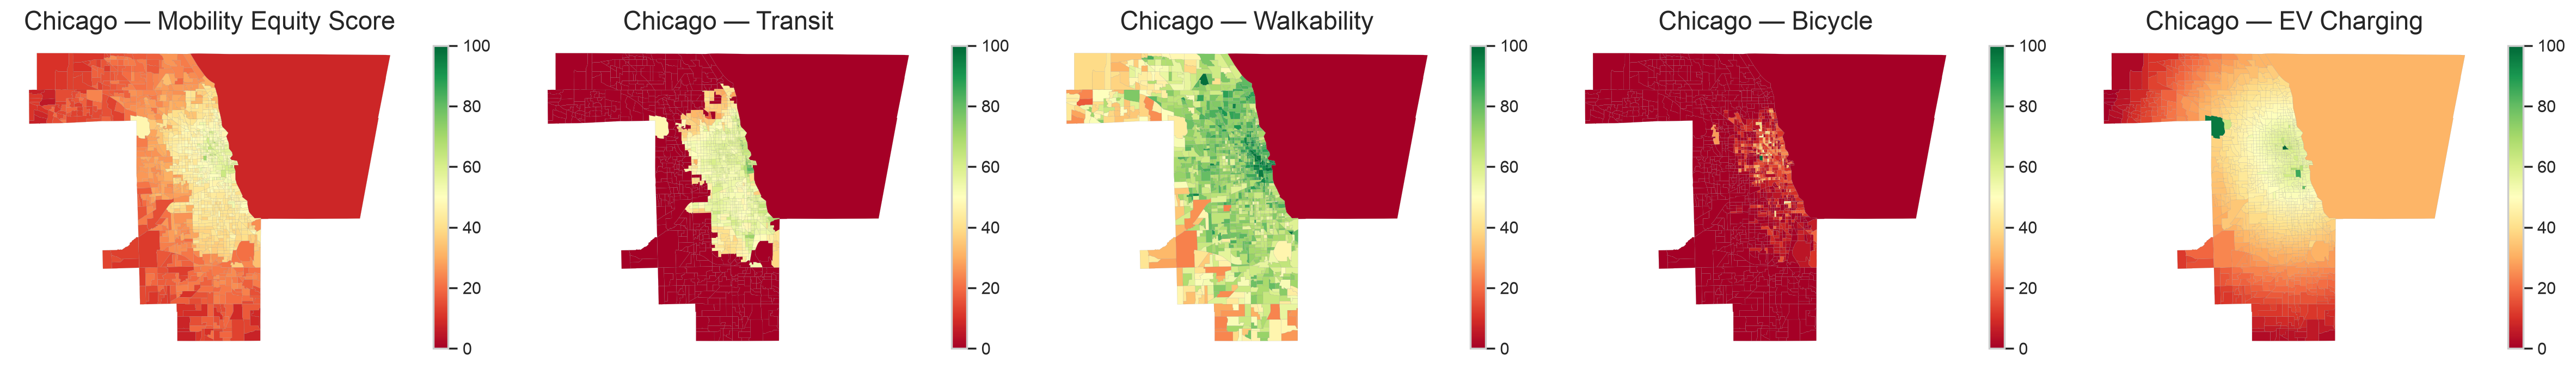
\includegraphics[width=\textwidth]{choropleth_chicago.png}\\[3pt]
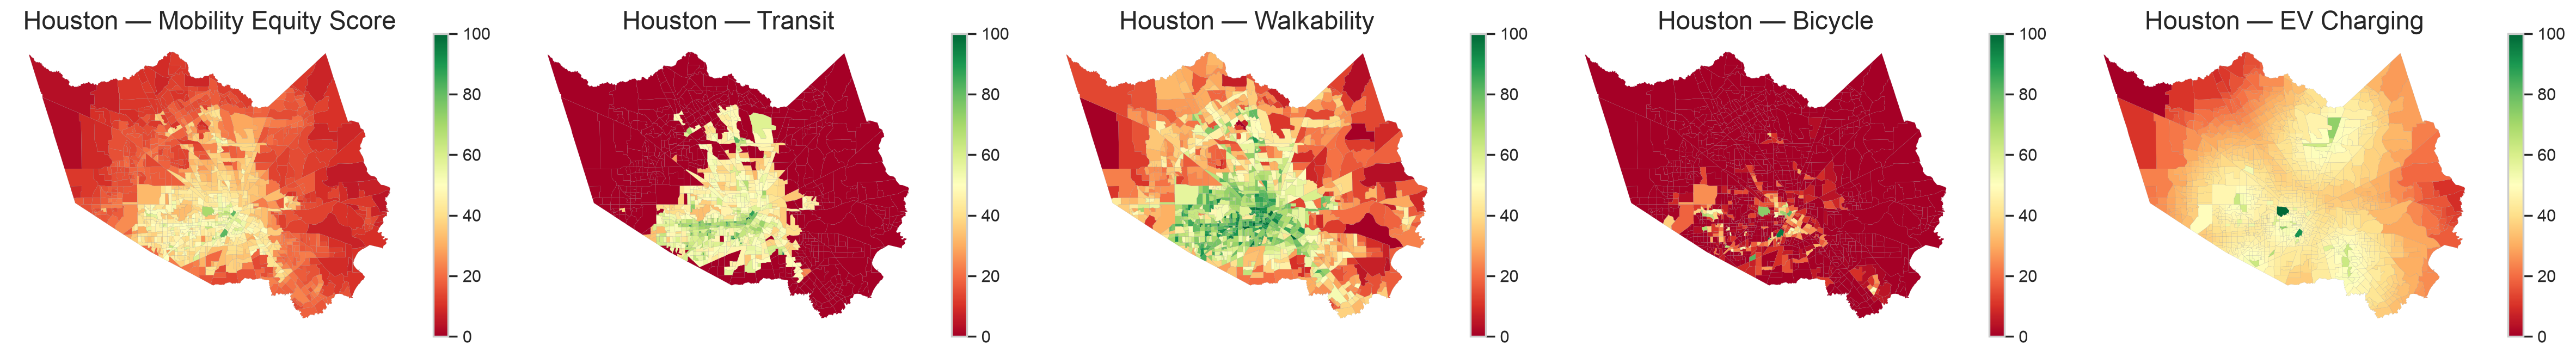
\includegraphics[width=\textwidth]{choropleth_houston.png}\\[3pt]
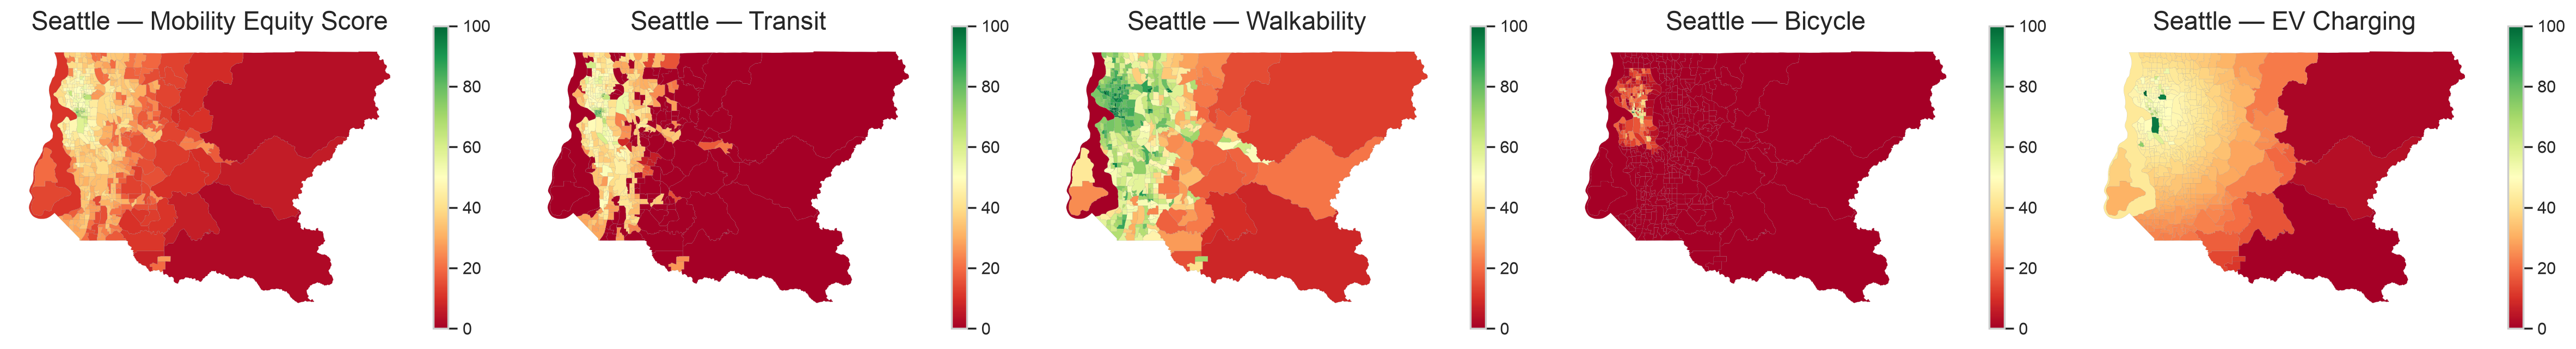
\includegraphics[width=\textwidth]{choropleth_seattle.png}
\caption{MES and sub-index choropleths (Chicago, Houston, Seattle). Green = better
served, red = worse. Walkability and transit concentrate centrally; dedicated
bicycle infrastructure is sparse citywide.}
\label{fig:choropleth}
\end{figure}

\subsection{Equity Correlation Analysis}
Table~\ref{tab:corr} reports the Pearson correlations. Three patterns hold across
all cities and are all statistically significant ($p<0.05$, 95\% CIs excluding
zero): the MES is (i) \emph{negatively} associated with median income
($r=-0.08$ to $-0.27$), (ii) \emph{positively} and strongly associated with the
share of zero-vehicle households ($r=0.41$ to $0.69$), and (iii) positively
associated with renter share ($r=0.53$ to $0.69$). The association with percent
non-white is positive but weak ($r=0.10$ to $0.14$). Descriptively, the MES
co-occurs with higher shares of car-free and renter households --- the dense
urban core; the raw negative income association is probed for confounding in
Sec.~4.7, where it largely disappears once urban form is controlled. All coefficients
are associational, not causal, and (as Sec.~4.7 shows) their significance is
overstated by spatial dependence. Figure~\ref{fig:corr} visualizes the full
correlation structure for Chicago. A Spearman rank check agrees in sign with every Pearson
coefficient in all three cities; the strong zero-vehicle and renter associations
remain strong under ranks, while the weaker income and non-white associations
attenuate --- indicating the latter are more sensitive to distributional outliers
and should be read cautiously. The four sub-indices show coherent but
non-redundant internal structure (mean inter-sub-index Pearson
$r = 0.45$--$0.62$, pairwise range $0.26$--$0.81$), i.e.\ related enough to form
a coherent composite yet distinct enough that each contributes non-redundant
information --- the appropriate validity evidence for a \emph{formative} index,
rather than a reflective-scale reliability statistic (RQ1).

\begin{table}[htbp]
\centering
\caption{Pearson correlation of the MES with demographic variables ($r$ [95\%
CI], all $p<0.05$).}
\label{tab:corr}
\small
\begin{tabularx}{\textwidth}{l Y Y Y}
\toprule
\textbf{Variable} & \textbf{Chicago} & \textbf{Houston} & \textbf{Seattle} \\
\midrule
Median income      & $-0.085$ $[-0.14,-0.03]$ & $-0.144$ $[-0.20,-0.09]$ & $-0.272$ $[-0.35,-0.19]$ \\
\% non-white       & $+0.140$ $[0.09,0.19]$   & $+0.097$ $[0.04,0.16]$   & $+0.102$ $[0.01,0.19]$ \\
\% zero-vehicle    & $+0.562$ $[0.52,0.60]$   & $+0.408$ $[0.36,0.46]$   & $+0.691$ $[0.64,0.73]$ \\
\% renter          & $+0.576$ $[0.54,0.61]$   & $+0.535$ $[0.49,0.58]$   & $+0.686$ $[0.64,0.73]$ \\
\bottomrule
\end{tabularx}
\end{table}

\begin{figure}[htbp]
\centering
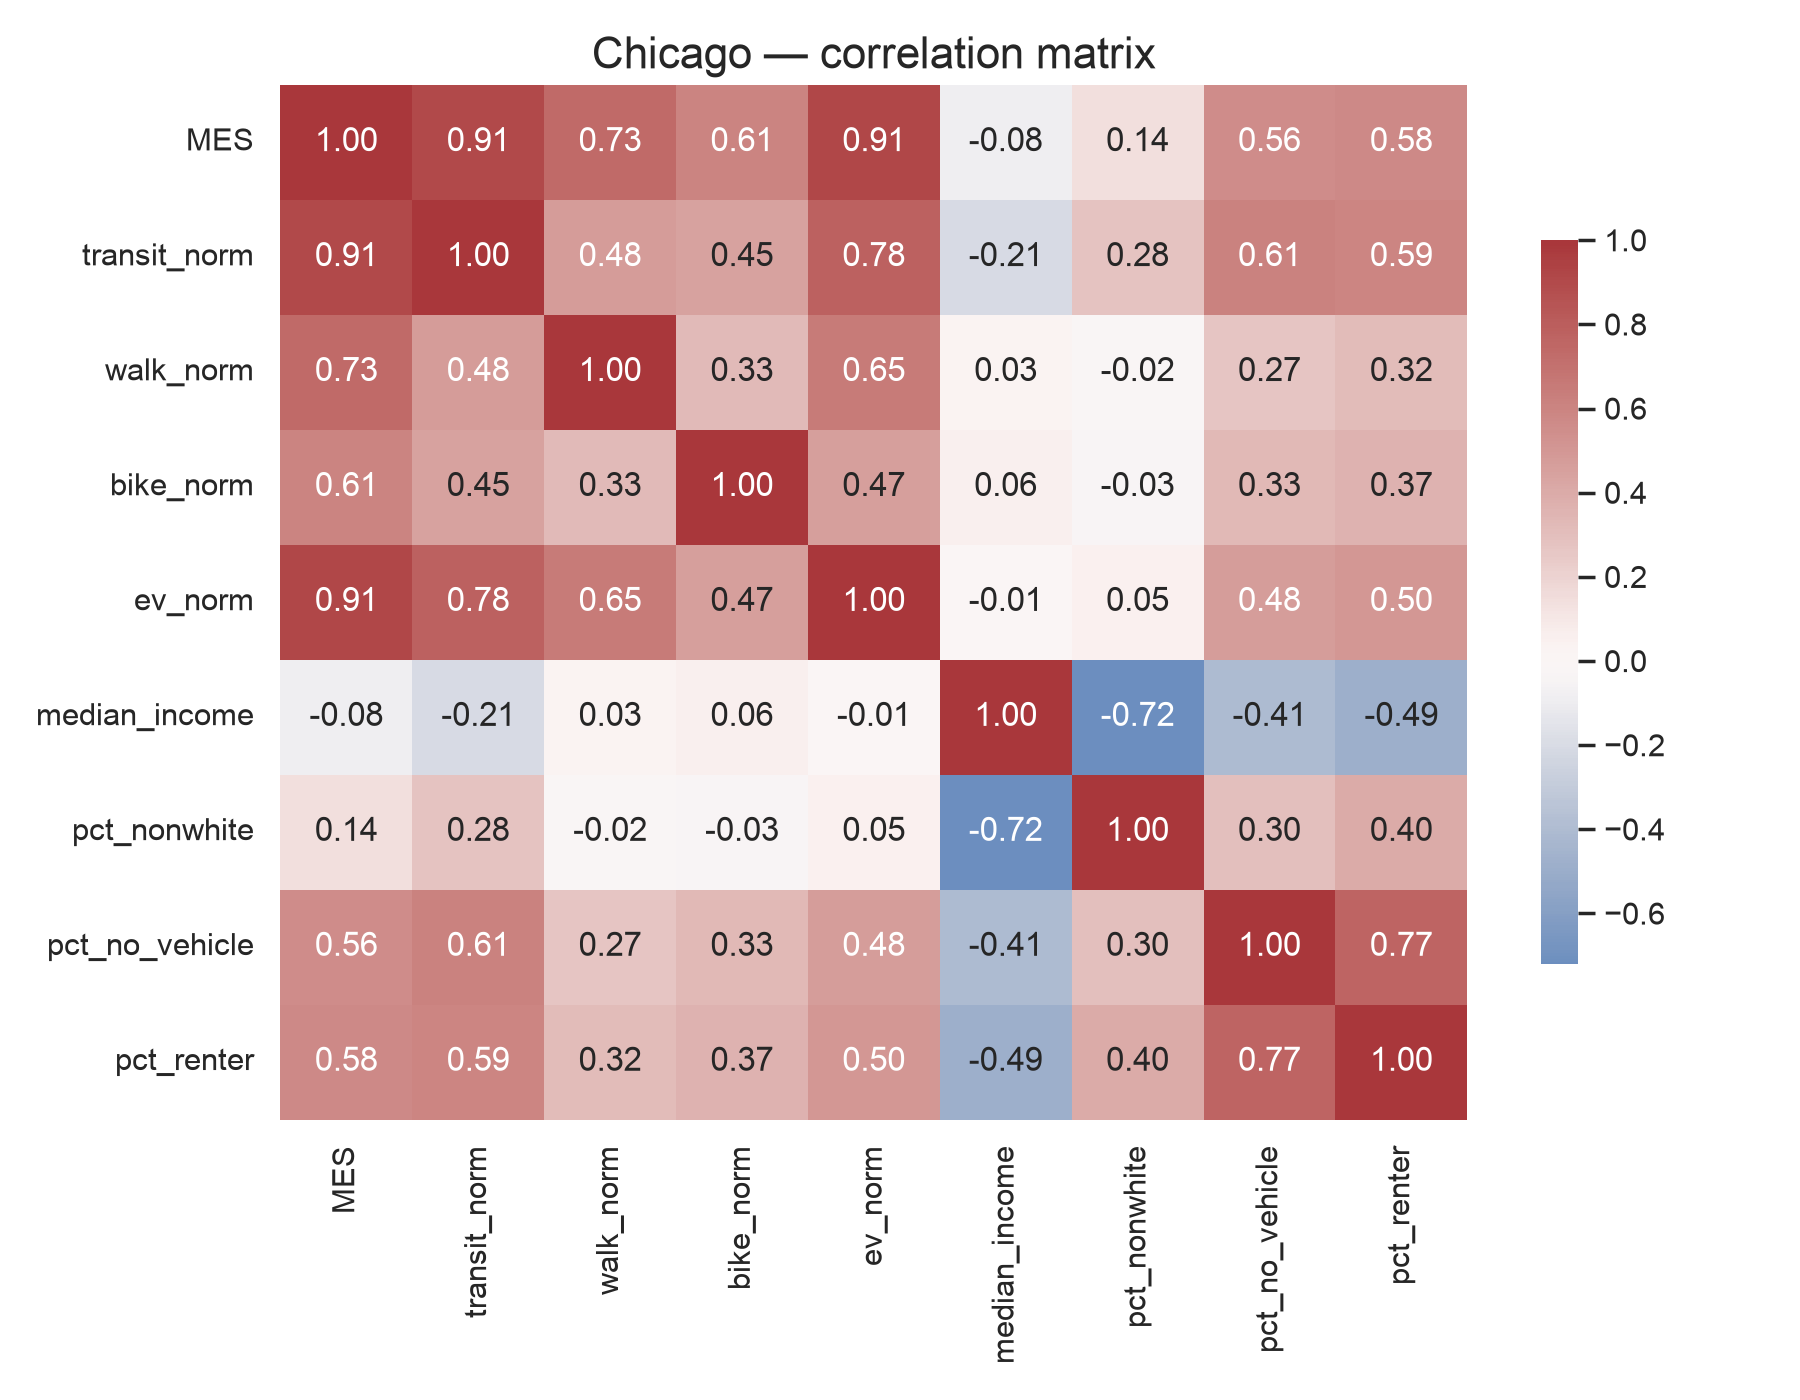
\includegraphics[width=0.72\textwidth]{corr_heatmap_chicago.png}
\caption{Chicago correlation matrix among the MES, its sub-indices, and
demographic variables.}
\label{fig:corr}
\end{figure}

\subsection{Spatial Autocorrelation}
The MES is strongly spatially clustered in every city (Table~\ref{tab:moran}):
global Moran's $I$ ranges from 0.82 (Seattle) to 0.92 (Chicago), all with
$p=0.001$ and large $z$-scores. Well-served and under-served tracts thus form
contiguous patches, not a random scatter --- confirming systematic, place-based
inequity. Local Moran's $I$ (Figure~\ref{fig:lisa}) locates the significant
low-low cold spots (peripheral, lower-supply clusters) that are the natural
targets for investment.

\begin{table}[htbp]
\centering
\caption{Global Moran's $I$ for the MES (queen contiguity, 999 permutations).}
\label{tab:moran}
\small
\begin{tabularx}{\textwidth}{l Y Y Y Y}
\toprule
\textbf{City} & \textbf{Moran's $I$} & \textbf{$z$-score} & \textbf{$p$-value} & \textbf{$n$} \\
\midrule
Chicago & 0.916 & 60.9 & 0.001 & 1{,}332 \\
Houston & 0.834 & 48.2 & 0.001 & 1{,}115 \\
Seattle & 0.820 & 31.0 & 0.001 & 495 \\
\bottomrule
\end{tabularx}
\end{table}

\begin{figure}[htbp]
\centering
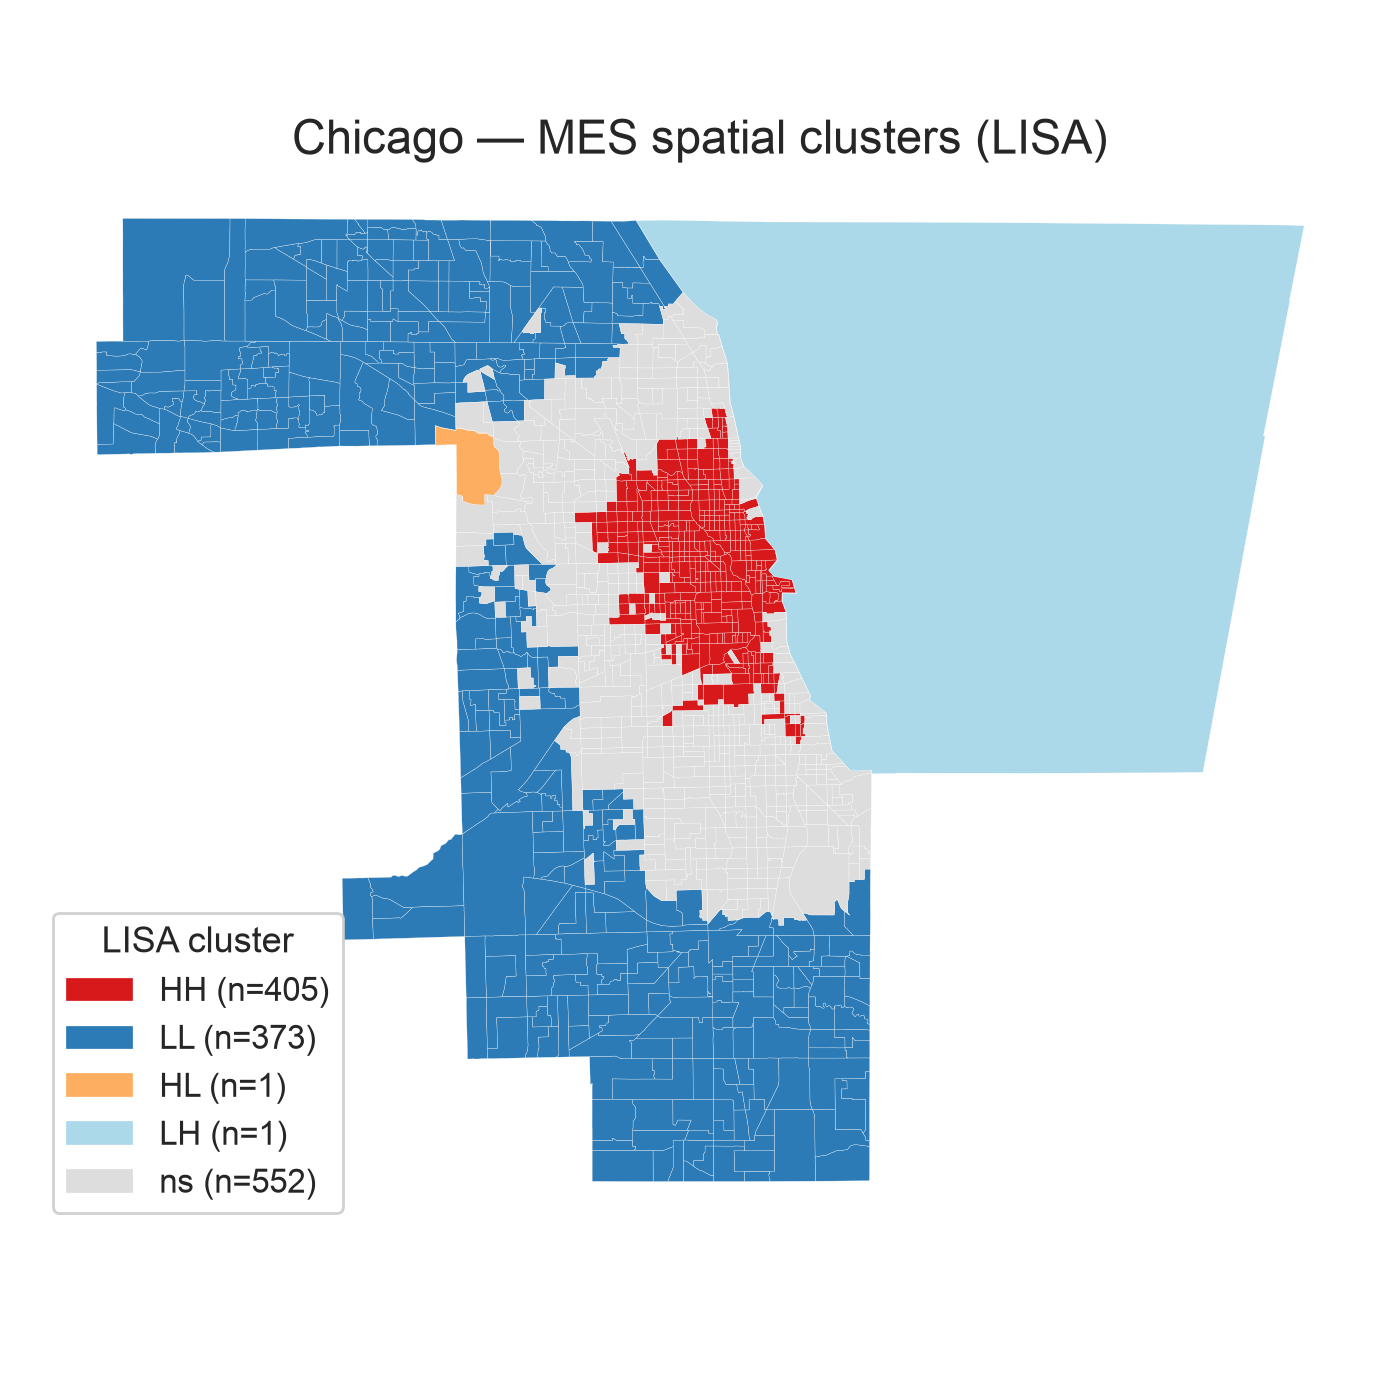
\includegraphics[width=0.32\textwidth]{lisa_chicago.png}\hfill
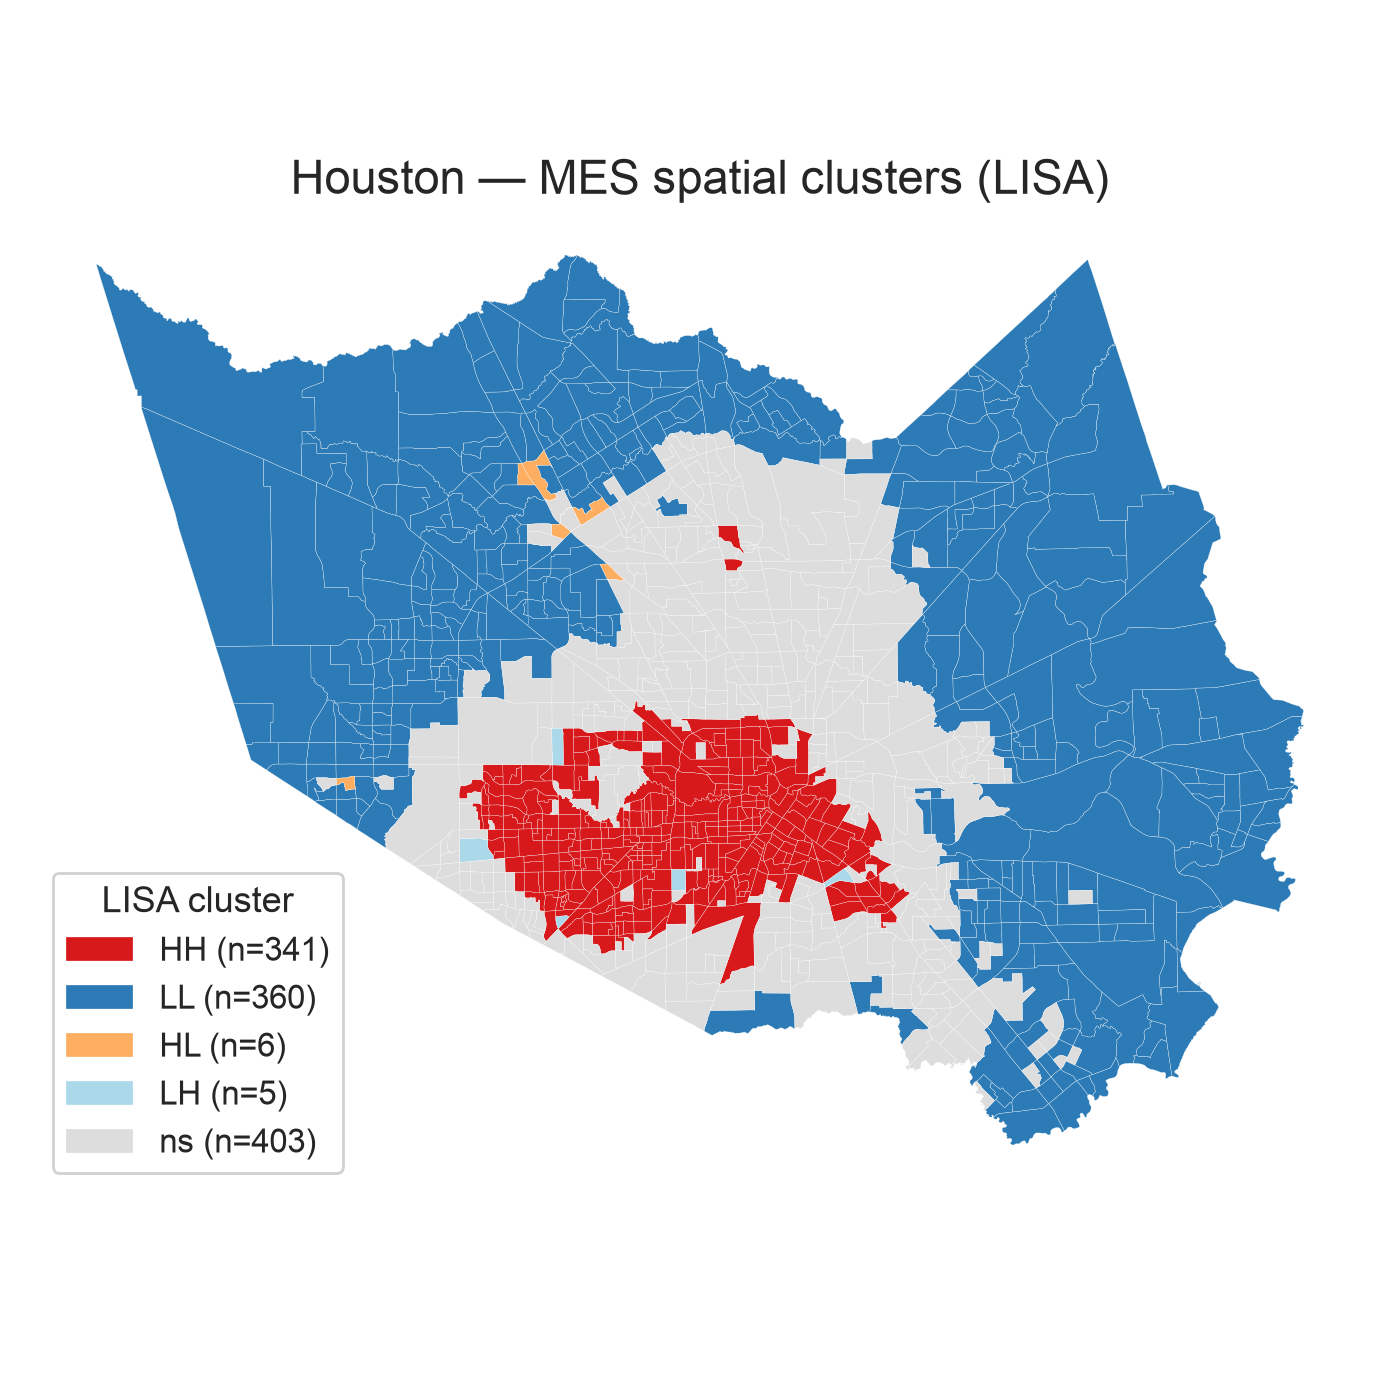
\includegraphics[width=0.32\textwidth]{lisa_houston.png}\hfill
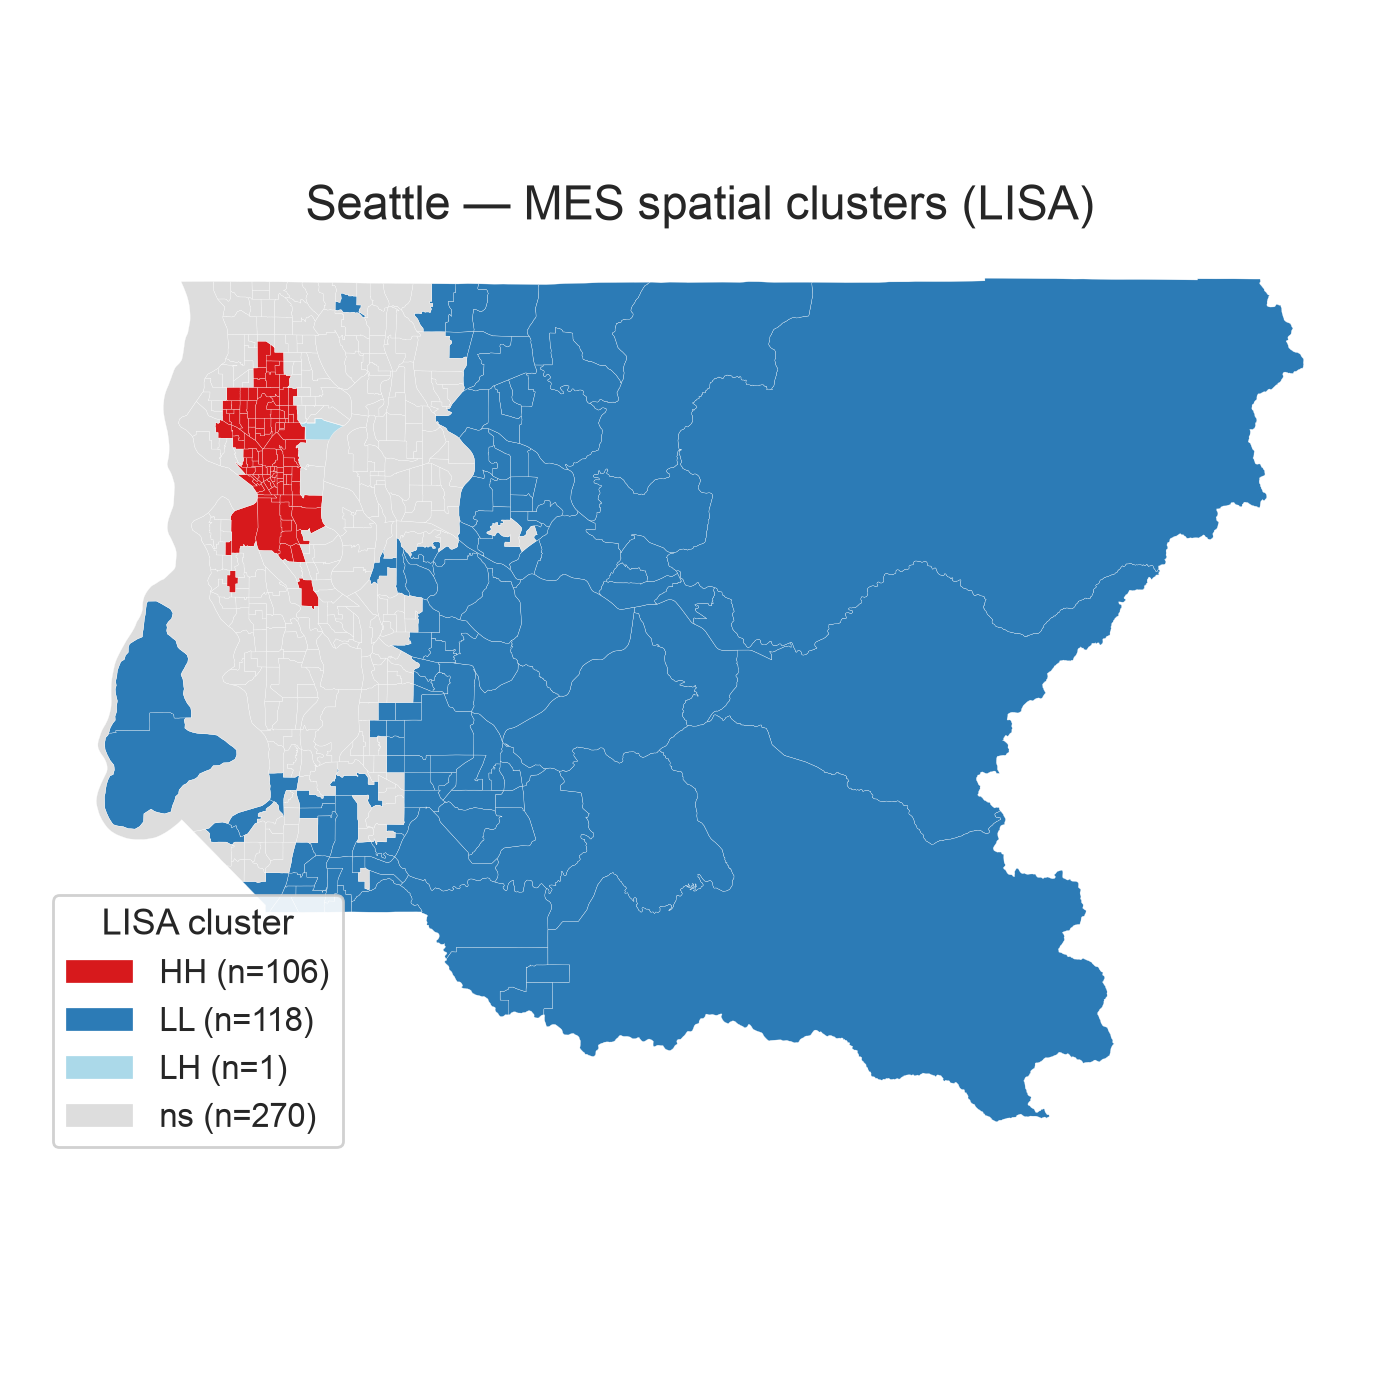
\includegraphics[width=0.32\textwidth]{lisa_seattle.png}
\caption{Local Moran's $I$ (LISA) clusters. Red = high-high (well-served cores),
blue = low-low (under-served cold spots).}
\label{fig:lisa}
\end{figure}

\subsection{Mobility-Desert Classification and Threshold Robustness}
Table~\ref{tab:sensitivity} shows the desert classification is robust to the
percentile threshold: moving from the 25th to the 20th or 30th percentile yields
Jaccard overlaps of $0.80$--$0.83$ with the baseline set (well above the
0.75 criterion), and the demographic profile of flagged tracts is stable. Notably,
the mean median income of desert tracts is \emph{high} in every city (Chicago
\$96.8k, Houston \$94.1k, Seattle \$157.4k), and their mean non-white share is
substantial (Chicago 52\%, Houston 64\%, Seattle 39\%) --- the deserts are
higher-income peripheries that nonetheless include large minority populations.

\begin{table}[htbp]
\centering
\caption{Desert-threshold sensitivity: Jaccard overlap with the 25th-percentile
baseline, and demographic profile of flagged tracts.}
\label{tab:sensitivity}
\small
\begin{tabularx}{\textwidth}{l c Y Y Y}
\toprule
\textbf{City} & \textbf{Threshold} & \textbf{Jaccard vs.\ 25th} & \textbf{Mean income (\$)} & \textbf{Mean \% non-white} \\
\midrule
Chicago & 20th / 30th & 0.80 / 0.83 & 97.1k / 98.2k & 51.4 / 51.2 \\
Houston & 20th / 30th & 0.80 / 0.83 & 95.6k / 94.2k & 63.0 / 64.9 \\
Seattle & 20th / 30th & 0.80 / 0.83 & 158.4k / 153.9k & 38.7 / 40.9 \\
\bottomrule
\end{tabularx}
\end{table}

\subsection{Cluster Typology}
Silhouette-selected K-means (Figure~\ref{fig:cluster}) yields interpretable
profiles (Table~\ref{tab:typology}). Chicago and Seattle resolve into two groups
--- a well-served multimodal core and a uniformly under-served periphery ---
while Houston resolves into three, adding a distinctive ``walk-rich, bike-poor''
class (537 tracts) that has moderate walkability and transit but almost no
cycling infrastructure. Across all cities the near-zero bicycle centroid confirms
that cycling is the systematically weakest dimension. The silhouette for the
selected $k$ is 0.48 (Chicago, $k{=}2$), 0.48 (Houston, $k{=}3$), and 0.41
(Seattle, $k{=}2$), and the partitions are perfectly reproducible across random
initializations (Sec.~4.7). Because $k$ differs across cities, similarly named
profiles are \emph{not} assumed to represent identical neighborhood structures;
cross-city comparison is by centroid shape, not by label.

\begin{table}[htbp]
\centering
\caption{K-means mobility typologies (centroid sub-index scores, 0--100).}
\label{tab:typology}
\small
\begin{tabularx}{\textwidth}{l Y r r r r}
\toprule
\textbf{City} & \textbf{Profile} & \textbf{Transit} & \textbf{Walk} & \textbf{Bike} & \textbf{EV} \\
\midrule
Chicago & Well-served / multimodal (868) & 53.3 & 73.5 & 8.2 & 49.7 \\
Chicago & Uniformly under-served (464)   & 0.5  & 58.9 & 0.1 & 25.8 \\
Houston & Walk-rich, bike-poor (537)     & 53.1 & 67.0 & 2.5 & 44.6 \\
Houston & Uniformly under-served (484)   & 1.1  & 29.2 & 0.7 & 34.5 \\
Houston & Well-served / multimodal (94)  & 55.0 & 71.5 & 38.5 & 46.7 \\
Seattle & Well-served / multimodal (170) & 52.4 & 82.4 & 20.6 & 50.4 \\
Seattle & Uniformly under-served (325)   & 23.6 & 54.0 & 0.3 & 34.9 \\
\bottomrule
\end{tabularx}
\end{table}

\begin{figure}[htbp]
\centering
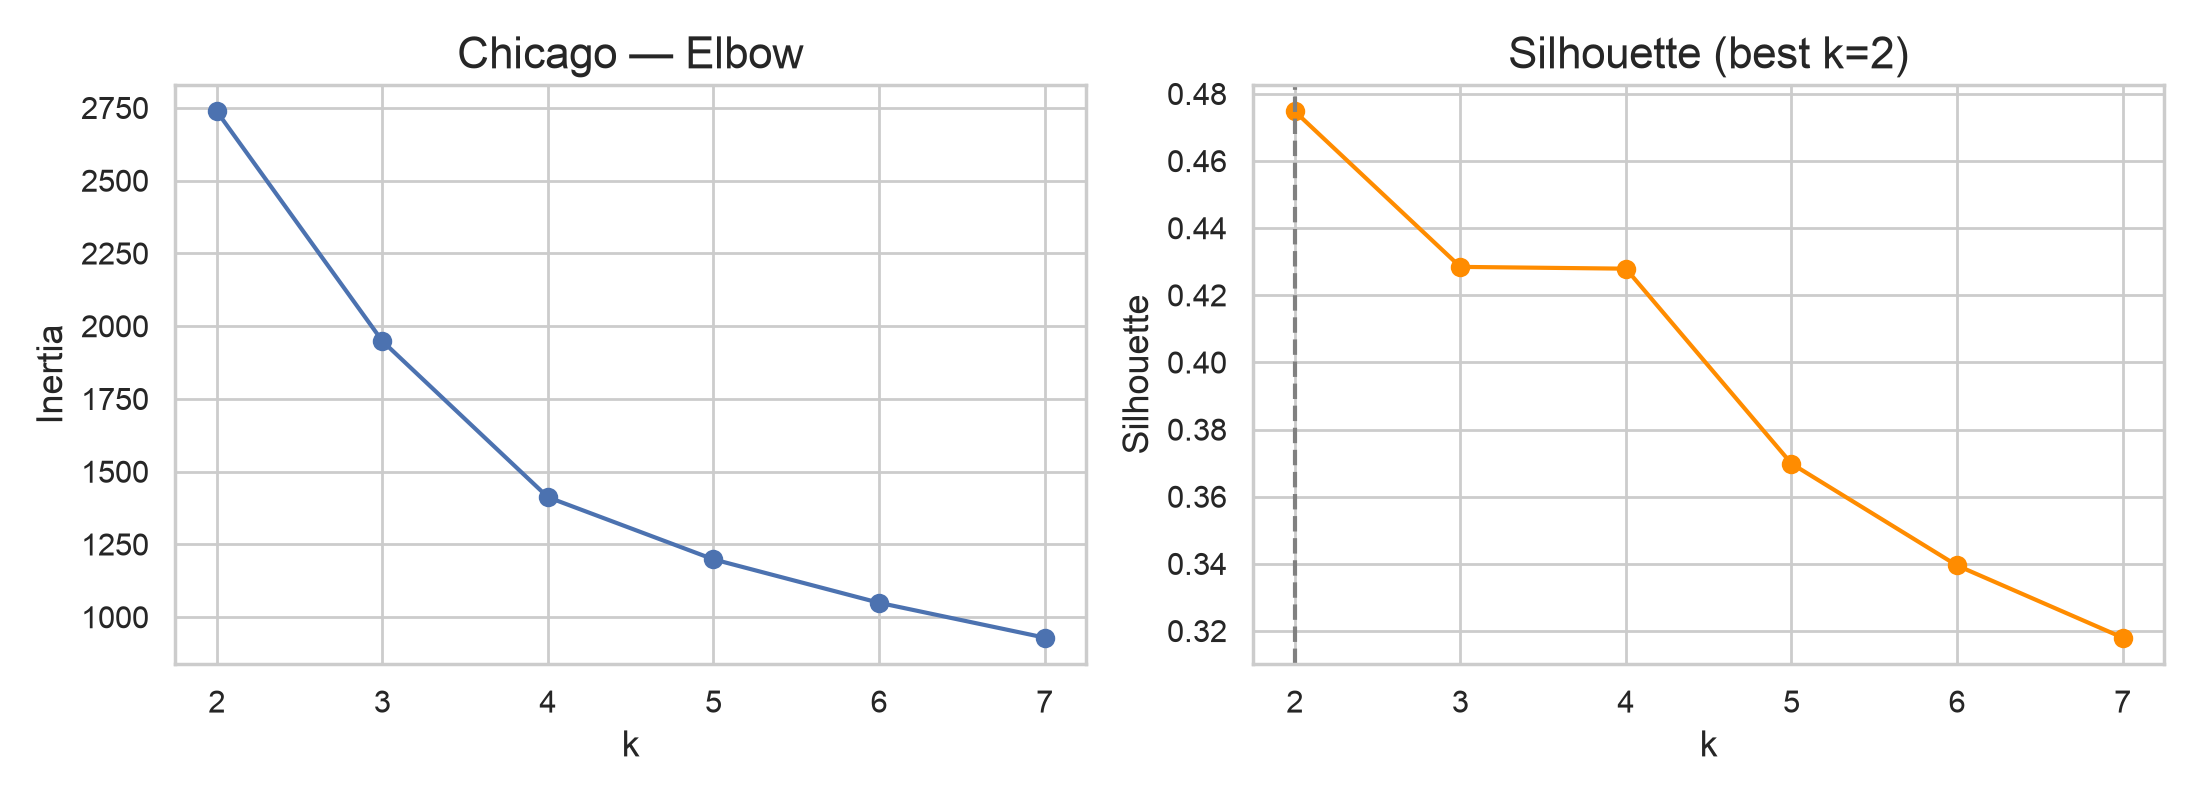
\includegraphics[width=0.8\textwidth]{clustering_chicago.png}
\caption{Elbow (inertia) and silhouette curves for Chicago; silhouette is
maximized at $k=2$.}
\label{fig:cluster}
\end{figure}

\subsection{Weighting Sensitivity}
The equal-weight baseline is treated as one scenario among several; entropy and
PCA weights are objective sensitivity scenarios, and the policy-priority
(expert-inspired) weights represent a plausible planner preference. The headline
is \emph{stability}: re-computing the MES under all four schemes leaves the
equity associations unchanged in sign and significance (Chicago shown ---
MES--renter $r\approx0.57$--$0.59$; MES--income negative and weak throughout).
The entropy scheme up-weights bicycle (0.68) because that sub-index has the
highest dispersion, yet even this extreme reweighting does not flip any sign
(RQ1).

\subsection{Robustness: Confounding, Spatial Dependence, and EV Data}
Because the bivariate correlations (Sec.~4.2) neither control for confounders nor
account for the strong spatial dependence (Sec.~4.3), four robustness checks were
run (Table~\ref{tab:robust}).

\emph{Urban-form confounding.} Adding population density and distance to the CBD
to an OLS of the MES on income sharply changes the income coefficient: it is
negative and significant bivariately in all three cities, but after controls it
becomes non-significant in Houston ($p=0.64$), reverses to weakly positive in
Chicago, and remains negative and significant only in Seattle ($p<10^{-20}$).
The apparent ``low-income cores are better served'' pattern is thus largely an
\emph{urban-form artifact} (density and centrality), not an income effect per se
--- except in Seattle, where it persists.

\emph{Spatial regression.} Fitting spatial-lag and spatial-error models (queen
contiguity) of the MES on income, renter share, zero-vehicle share, density, and
CBD distance, the error model is preferred for Chicago and the lag model for
Houston and Seattle (by AIC). Once spatial dependence is modelled, the income
association is negligible in Chicago/Houston and modest-negative in Seattle,
corroborating the OLS result and confirming that ordinary significance was
overstated.

\emph{Clustering stability.} Across five random initializations the K-means
partition is perfectly reproducible in every city (mean Adjusted Rand
Index $=1.00$; silhouette $0.41$--$0.48$), so the typologies are not seed
artefacts.

\emph{EV data.} Recomputing a three-dimension MES without the (OSM-sourced) EV
layer leaves the principal findings intact on every axis: the correlations with
income, renter share, and zero-vehicle share all move by $|\Delta r|\leq 0.05$;
the mobility-desert set overlaps the four-dimension set by a Jaccard of
$0.71$--$0.92$; and the spatial clustering is essentially unchanged (Moran's $I$
of $0.77$--$0.87$ versus $0.82$--$0.92$). The conclusions therefore do not depend
on the least-certain dimension.

\begin{table}[htbp]
\centering
\caption{Robustness checks. Income associations attenuate under urban-form
controls and spatial regression (except Seattle); clustering is stable and the
EV layer is non-decisive.}
\label{tab:robust}
\small
\begin{tabularx}{\textwidth}{l Y Y l c c}
\toprule
\textbf{City} & \textbf{MES--income, bivariate} & \textbf{+ urban-form controls} & \textbf{Spatial (AIC)} & \textbf{Cluster ARI} & \textbf{EV max $|\Delta r|$} \\
\midrule
Chicago & $-$, $p{=}.002$ & $+$, weak & error & 1.00 & 0.025 \\
Houston & $-$, $p{<}.001$ & n.s.\ ($p{=}.64$) & lag & 1.00 & 0.009 \\
Seattle & $-$, $p{<}.001$ & $-$, $p{<}.001$ & lag & 1.00 & 0.053 \\
\bottomrule
\end{tabularx}
\end{table}

\subsection{Dashboard Demonstration}
The interactive dashboard (Figure~\ref{fig:dash}) renders the tract-level MES and
any sub-index, supports click-through inspection (score, city percentile,
sub-index bars versus the city median, and demographics), and compares the
equity gap across cities. It is the dissemination layer for the results above,
not a separate analysis.

\begin{figure}[htbp]
\centering
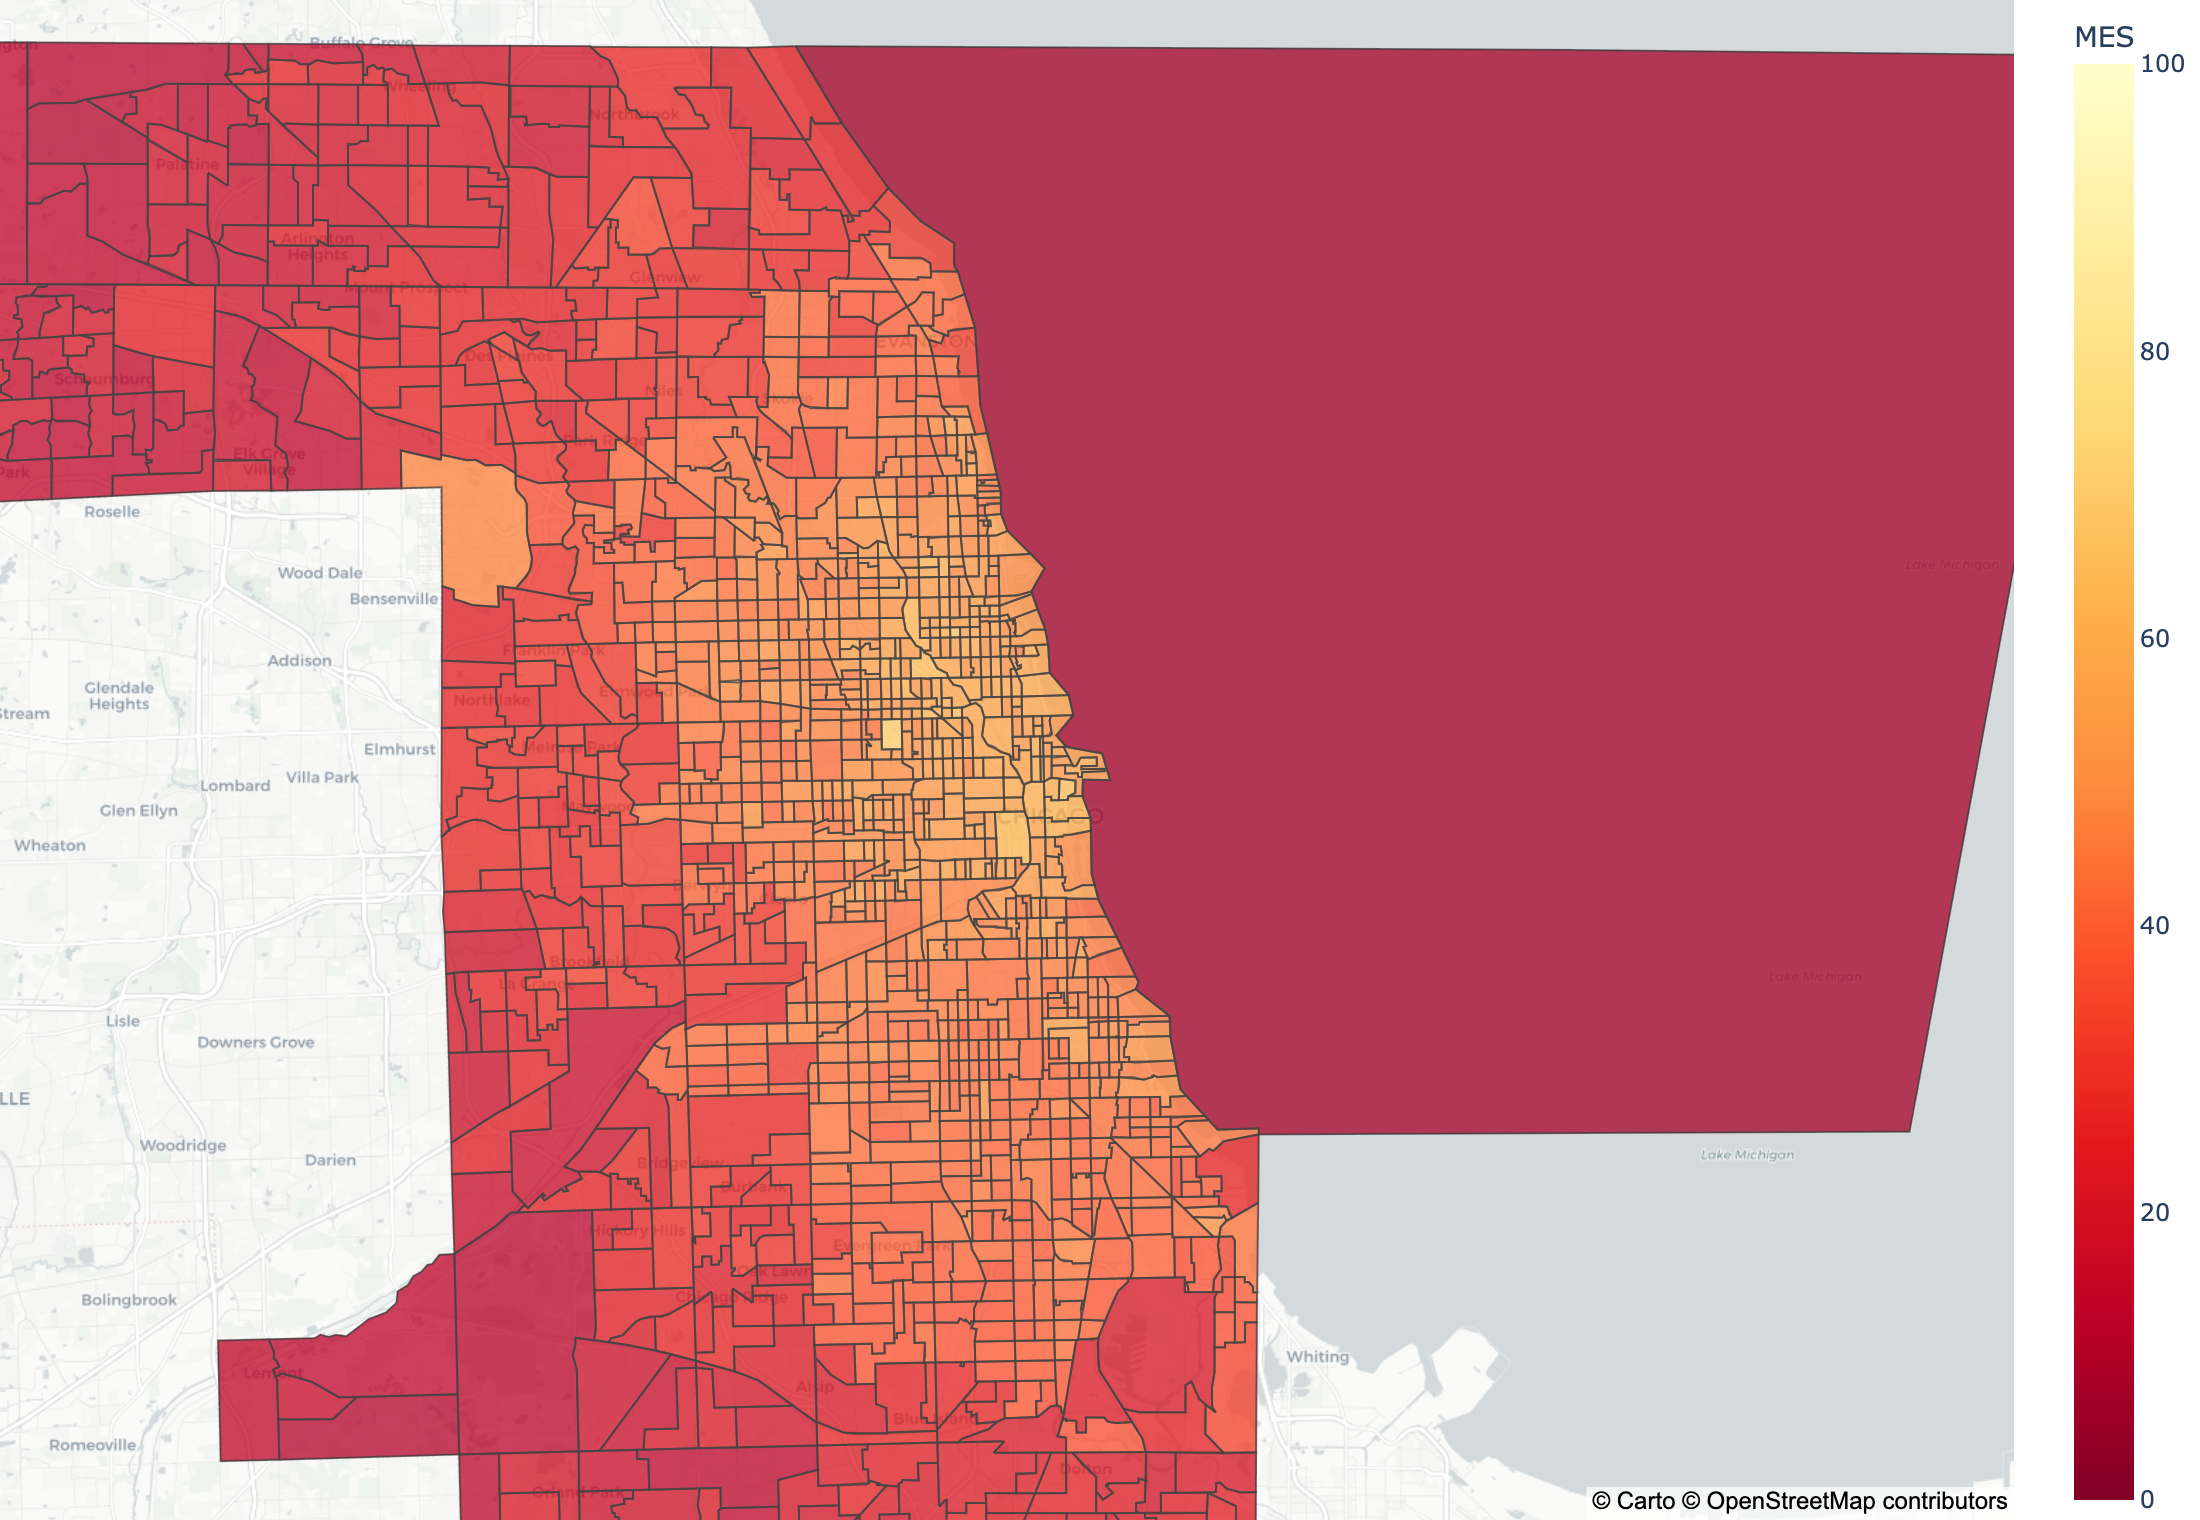
\includegraphics[width=0.62\textwidth]{dashboard_map_chicago.png}\\[4pt]
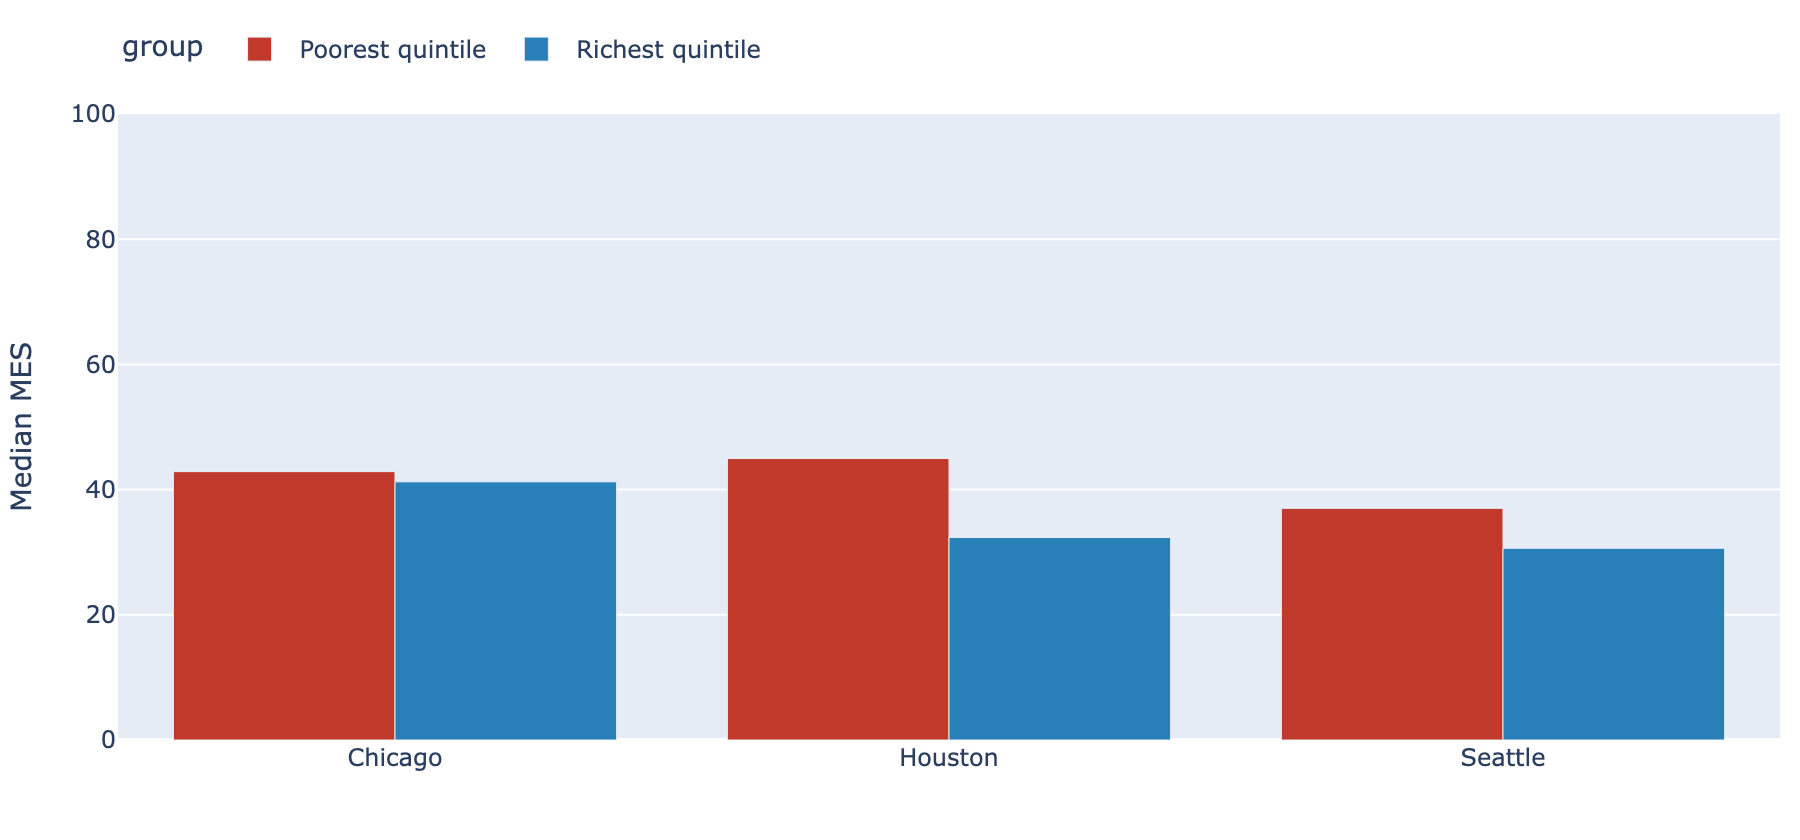
\includegraphics[width=0.72\textwidth]{dashboard_equity_gap.png}
\caption{Dashboard: Chicago MES choropleth (top) and the city equity-gap panel
(median MES of the poorest versus richest income quintile, bottom).}
\label{fig:dash}
\end{figure}

% ============================== CHAPTER 5 ==============================
\section{Discussion and Conclusions}

\subsection{What the Data Demonstrate}
This chapter deliberately separates what the analysis \emph{demonstrates} from
what it \emph{infers}. Four results are demonstrated and robust across all three
cities. (1) The MES is strongly spatially clustered (Moran's $I=0.82$--$0.92$):
supply inequity is structural and place-based, not scattered. (2) The MES is
positively associated with car-free and renter shares (associational; the
ordinary significance is corrected via spatial regression, Sec.~4.7). (3) The
bivariate \emph{negative} MES--income association is largely explained by urban
form --- it does not survive density/centrality controls or spatial regression
except in Seattle --- so it must not be read as an income effect per se. (4) The
composite is well-behaved: its four sub-indices are related but non-redundant,
results are stable across weighting schemes, the clusters are perfectly
reproducible (ARI $=1.0$), and the findings are insensitive to the EV layer.
Bicycle infrastructure is the weakest dimension everywhere, defining a recurring
``walk-rich, bike-poor'' neighborhood type.

\subsection{What We Infer: A Supply--Need Reframing}
The following is interpretation, not demonstration. Because supply-side
infrastructure co-occurs with density --- and therefore with car-free and renter
populations --- the equity question is best framed, associationally, as a
supply--\emph{need} mismatch: the MES measures supply, while car-free and renter
shares proxy need; travel demand itself is \emph{not} modelled here. Where dense
cores are well supplied, the residual concern is plausibly service \emph{quality}
and \emph{affordability}, which supply counts do not capture; where higher-income
peripheries score low, their residents are typically car-owning, so low supply is
likely less acute --- \emph{except} for the car-free and minority households
embedded in those peripheries (the Chicago/Houston desert tracts are 52--64\%
non-white), who plausibly face the widest supply--need gap. Compounded deserts and
LISA cold spots locate those tracts and are where the framework most plausibly
adds policy value. Seattle, where a negative income gradient persists under
controls, is the one city that may warrant a closer income-specific look.

\subsection{Implications}
For practitioners, the MES operationalizes the Justice40 mandate~\cite{argonne2022}
at neighborhood resolution: it ranks tracts, distinguishes single- from
multi-dimension deficits, and --- via the typology --- prescribes
\emph{differentiated} interventions (e.g., cycling investment for the
``walk-rich, bike-poor'' class; first/last-mile transit for uniformly
under-served peripheries). Because the pipeline is open and reproducible, any city
with GTFS and open data can generate the same diagnostics.

\subsection{Limitations}
Five limitations bound the conclusions. (1) \emph{Supply-side only}: the MES
measures infrastructure present, not realized accessibility, service quality,
affordability, or travel behavior. (2) \emph{EV data}: the EV sub-index uses
community-maintained OpenStreetMap charging points --- a reachable but
\emph{lower-bound} proxy for the authoritative DOE/NREL AFDC inventory, which was
unavailable on the development network; EV results should be read as
conservative and are the least certain of the four dimensions. (3)
\emph{Within-city normalization}: the MES is relative to each city, so cross-city
\emph{levels} are not directly comparable (within-city patterns and correlations
are valid). (4) \emph{Cross-sectional, three cities}: the analysis is a single
snapshot for three metros and is not yet generalizable nationally. (5)
\emph{Inferential}: because the MES is strongly spatially autocorrelated
(Moran's $I\approx0.9$), ordinary correlation $p$-values are optimistic; we
therefore report spatial-lag/error models and urban-form controls (Sec.~4.7), which
substantially attenuate the income association. Residual caveats are that the
associations are ecological (tract-level, not individual-level) and that
confounders beyond density and centrality are not modelled.

\subsection{Future Research}
Priorities are: extending to the Phase-2 cities (Phoenix, Atlanta, Detroit) and
beyond for national generalizability; substituting authoritative AFDC EV data and
adding transit \emph{service quality} (headway reliability, e.g.\ from the FTA
National Transit Database); layering EPA EJScreen environmental-justice indicators
alongside the demographic cross-tabs; and, most directly, developing a
\emph{demand-adjusted MES} that combines infrastructure supply with transportation
need (e.g., zero-vehicle households and jobs reachable within a travel-time budget)
so that the supply--need relationship can be modelled rather than inferred.
A longitudinal extension would then measure whether targeted investment narrows
the gaps the MES identifies.

\subsection{Answering the Research Questions}
The four research questions of Sec.~1.3 are answered directly by the results:
\begin{itemize}[leftmargin=1.4em,itemsep=1pt]
\item \textbf{RQ1 (measurement).} Yes --- the four open datasets integrate into a
coherent, non-redundant composite (inter-sub-index $r=0.45$--$0.62$) whose equity
associations are stable in sign and significance across equal, entropy, PCA, and
policy-priority weights (Sec.~4.2, Sec.~4.6).
\item \textbf{RQ2 (distribution).} About a quarter of tracts are deserts \emph{by
construction}, but the informative results are that the classification is stable
(Jaccard $0.80$--$0.83$ across thresholds), spatially concentrated in peripheral
cold spots, and compounded (low on $\geq2$ dimensions) in 13--23\% of tracts
(Sec.~4.4, Sec.~4.5).
\item \textbf{RQ3 (equity).} The MES is positively associated with car-free
($r=0.41$--$0.69$) and renter ($r=0.53$--$0.69$) shares and negatively with income
($r=-0.08$ to $-0.27$); the income association is largely urban-form-driven and
survives density/centrality controls and spatial regression only in Seattle
(Sec.~4.2, Sec.~4.7).
\item \textbf{RQ4 (spatial structure and typology).} The MES is strongly spatially
clustered (Moran's $I=0.82$--$0.92$, $p<0.001$) with mapped low-low cold spots,
and silhouette-selected K-means recovers two-to-three reproducible neighborhood
profiles per city (ARI $=1.00$) (Sec.~4.3, Sec.~4.5).
\end{itemize}

\subsection{Conclusion}
This project delivers an integrated, transparent, and reproducible measure of
multi-modal mobility supply at the neighborhood scale, and uses it to show that
mobility infrastructure in three major U.S. cities is spatially concentrated in
dense, central tracts --- with the apparent income gradient largely attributable
to urban form once controls and spatial regression are applied. The equity
question is therefore reframed, associationally, as a supply--\emph{need}
mismatch best examined through compounded deserts and cold spots. The open
pipeline and dashboard make the method immediately transferable to other cities.

% ============================== REFERENCES ==============================
% (thebibliography emits its own "References" heading)
\addcontentsline{toc}{section}{References}
\small
\begin{thebibliography}{99}
\setlength{\itemsep}{1pt}

\bibitem{aman2020} J. J. Aman and J. Smith-Colin, ``Transit deserts: Equity analysis of public transit accessibility,'' \textit{Journal of Transport Geography}, vol.~89, p.~102869, 2020.
\bibitem{urban2022} Urban Institute, ``Redefining Walkability: A Neighborhood-Level Analysis,'' Urban Institute, Washington, DC, 2022.
\bibitem{lou2025} J. Lou, A. Chandra, and M. Gordon, ``Equity and reliability of public electric vehicle charging stations in the United States,'' \textit{Nature Communications}, vol.~16, p.~4201, 2025.
\bibitem{ahmed2024} S. Ahmed, Z. Sultana, and M. Rahman, ``A systematic review of bicycle infrastructure design principles within urban bikeability indices,'' \textit{Sustainability}, vol.~17, no.~14, p.~6409, 2024.
\bibitem{ermagun2020} A. Ermagun and N. Tilahun, ``Transit equity and job accessibility,'' \textit{Transportation Research Part A}, vol.~134, pp.~191--204, 2020.
\bibitem{maharjan2024} S. Maharjan, F. Janatabadi, and A. Ermagun, ``Spatial inequity of transit and automobile access gap across America for underserved populations,'' \textit{Transportation Research Record}, vol.~2678, no.~1, pp.~674--690, 2024.
\bibitem{argonne2022} Argonne National Laboratory, ``Electric Vehicle Charging Equity Considerations,'' U.S. Department of Energy, 2022.
\bibitem{epa2024} U.S. EPA, ``Smart Location Mapping and National Walkability Index,'' EPA, 2024.
\bibitem{sustrans2023} Sustrans, ``Cycling and Walking Investment Strategy: Equity in Active Travel Infrastructure,'' Sustrans, Bristol, UK, 2023.
\bibitem{albashir2024} A. Albashir et al., ``15min City Score Toolkit: Urban Walkability Analytics,'' Transform Transport Working Papers, Zenodo, 2024.
\bibitem{chenli2024} X. Chen and Y. Li, ``Electric vehicle charging equity and accessibility: A U.S. policy analysis,'' \textit{Transportation Research Part D}, vol.~118, p.~103748, 2024.
\bibitem{urbanSITE2025} Urban Institute, ``Spending on Infrastructure toward Equity (SITE) Tool,'' 2025.
\bibitem{oliverwyman2024} Oliver Wyman Forum, ``2024 Urban Mobility Readiness Index,'' 2024.
\bibitem{pandey2025} B. Pandey, C. Brelsford, and K. C. Seto, ``Rising infrastructure inequalities accompany urbanization and economic development,'' \textit{Nature Communications}, vol.~16, p.~1082, 2025.
\bibitem{boeing2017} G. Boeing, ``OSMnx: New methods for acquiring, constructing, analyzing, and visualizing complex street networks,'' \textit{Computers, Environment and Urban Systems}, vol.~65, pp.~126--139, 2017.
\bibitem{nardo2008} M. Nardo, M. Saisana, A. Saltelli, et al., \textit{Handbook on Constructing Composite Indicators: Methodology and User Guide}. OECD/JRC, 2008.
\bibitem{anselin1995} L. Anselin, ``Local Indicators of Spatial Association---LISA,'' \textit{Geographical Analysis}, vol.~27, no.~2, pp.~93--115, 1995.
\bibitem{rousseeuw1987} P. J. Rousseeuw, ``Silhouettes: A graphical aid to the interpretation and validation of cluster analysis,'' \textit{Journal of Computational and Applied Mathematics}, vol.~20, pp.~53--65, 1987.

\end{thebibliography}

\end{document}
